\documentclass{neu_handout}
\usepackage{url}
\usepackage{amssymb}
\usepackage{amsmath}
\usepackage{marvosym}
\usepackage{graphicx}
\usepackage[pdftex]{graphicx}
\usepackage{subfigure}
\graphicspath{ {images/} }
\everymath{\displaystyle}

% Professor/Course information
\title{Homework 4}
\author{Emily Dutile}
\date{March 2018}
\course{CS7295}{Info Viz}

\begin{document}

The dataset used for this homework can be found here \footnote{\url{https://drive.google.com/drive/folders/1UzuC3T8Y5M2DC-Q-d-DWimKJ72vuXjdu}}.

\section*{1 Dear Data}

\subsection*{1.1 My Visualization}

In order to visualization my question, I decided to keep track of all of the things that I saw in a day that were beautiful to me. I thought I could gather some substantial data with the following categories: people, animals, plants, weather, objects, art, music, language, literature, and happiness. People, consisted of individuals like my boyfriend, friends at school and outside of school, and family. Although not necessarily weather, I did incorporate things such as "sunsets" in weather, and literature could also consist of articles or short stories rather than just novels. Every tally represented one of these moments. To discover where I might "see more beauty" during my day, I decided to keep track of the location of where I was at the time. Giving insight into what day it was also gave me an interesting idea to see if I think I see more beautiful things during the weekend or during my routinely day.\\

In order to think more abstractly and not fall back on a bar chart or some standard visualization, I thought it was best to group different types of beauty into some category was necessary to give some meaning to the data. I also thought that adding location and the day added another more granular level of detail and could add some interesting interpretation afterwards.

\begin{figure}[h]
\centering
{
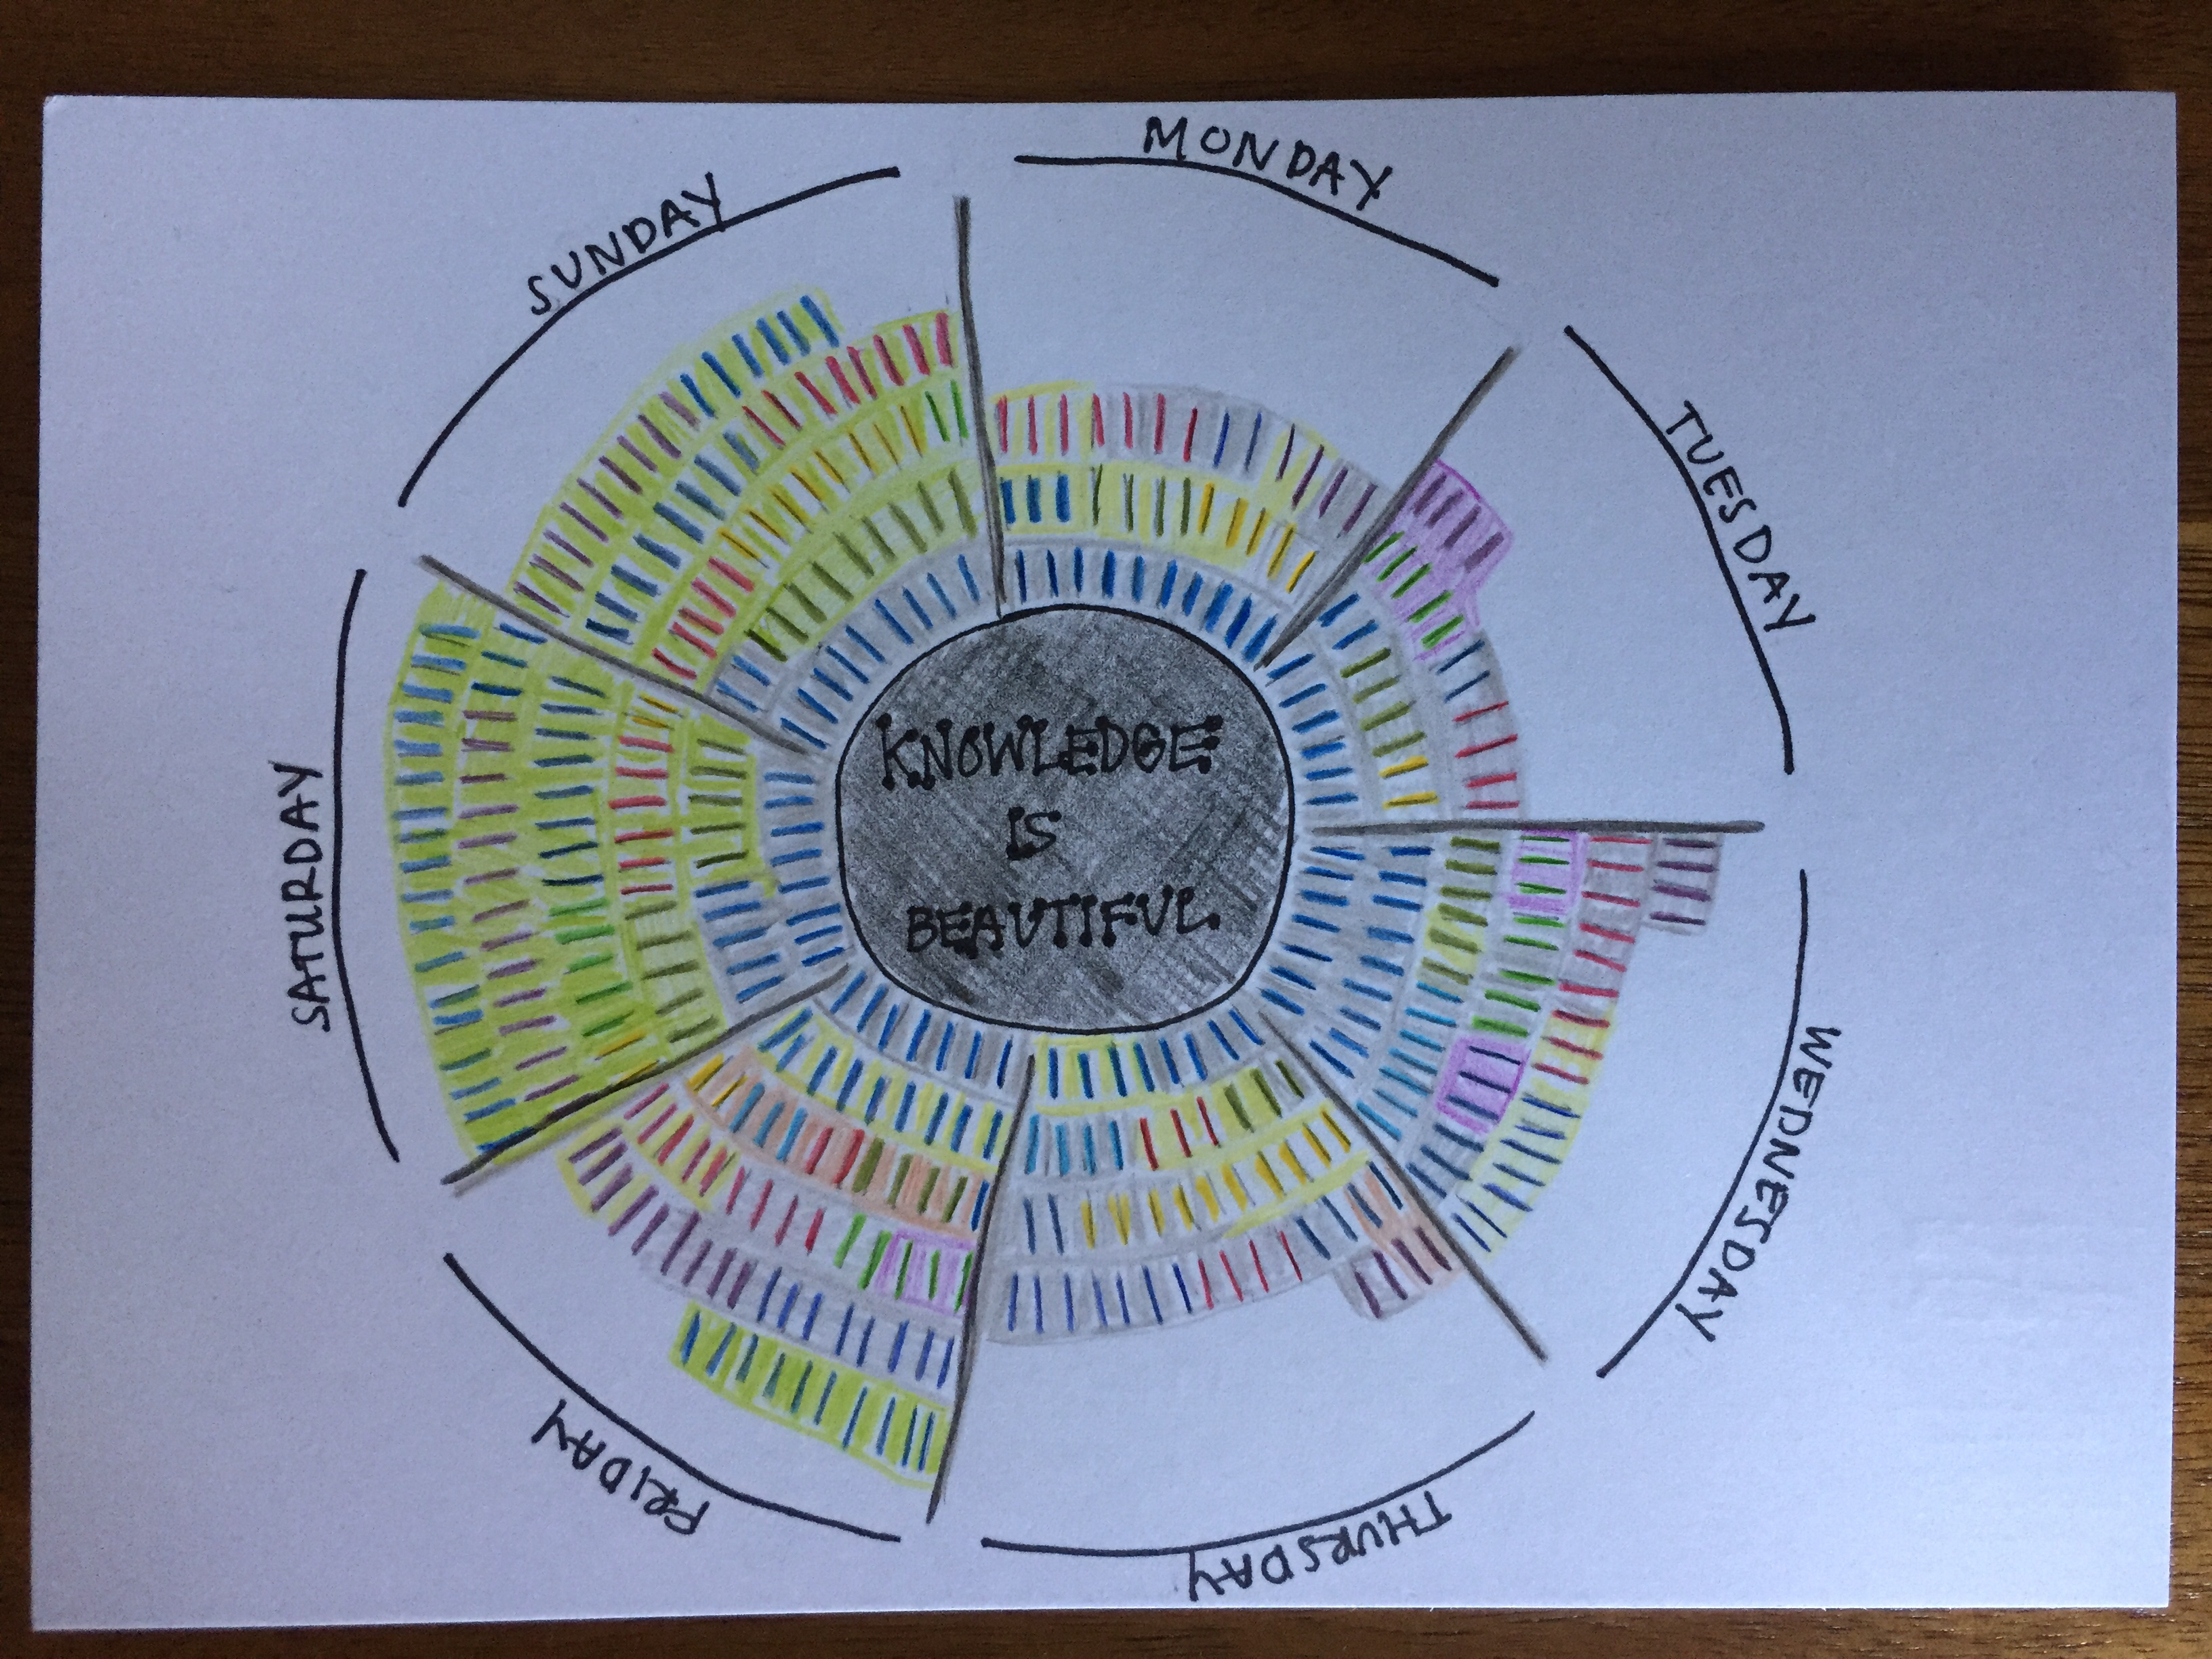
\includegraphics[width=0.4\linewidth]{myviz1}
}
\end{figure}

\begin{figure}[h]
\centering
{
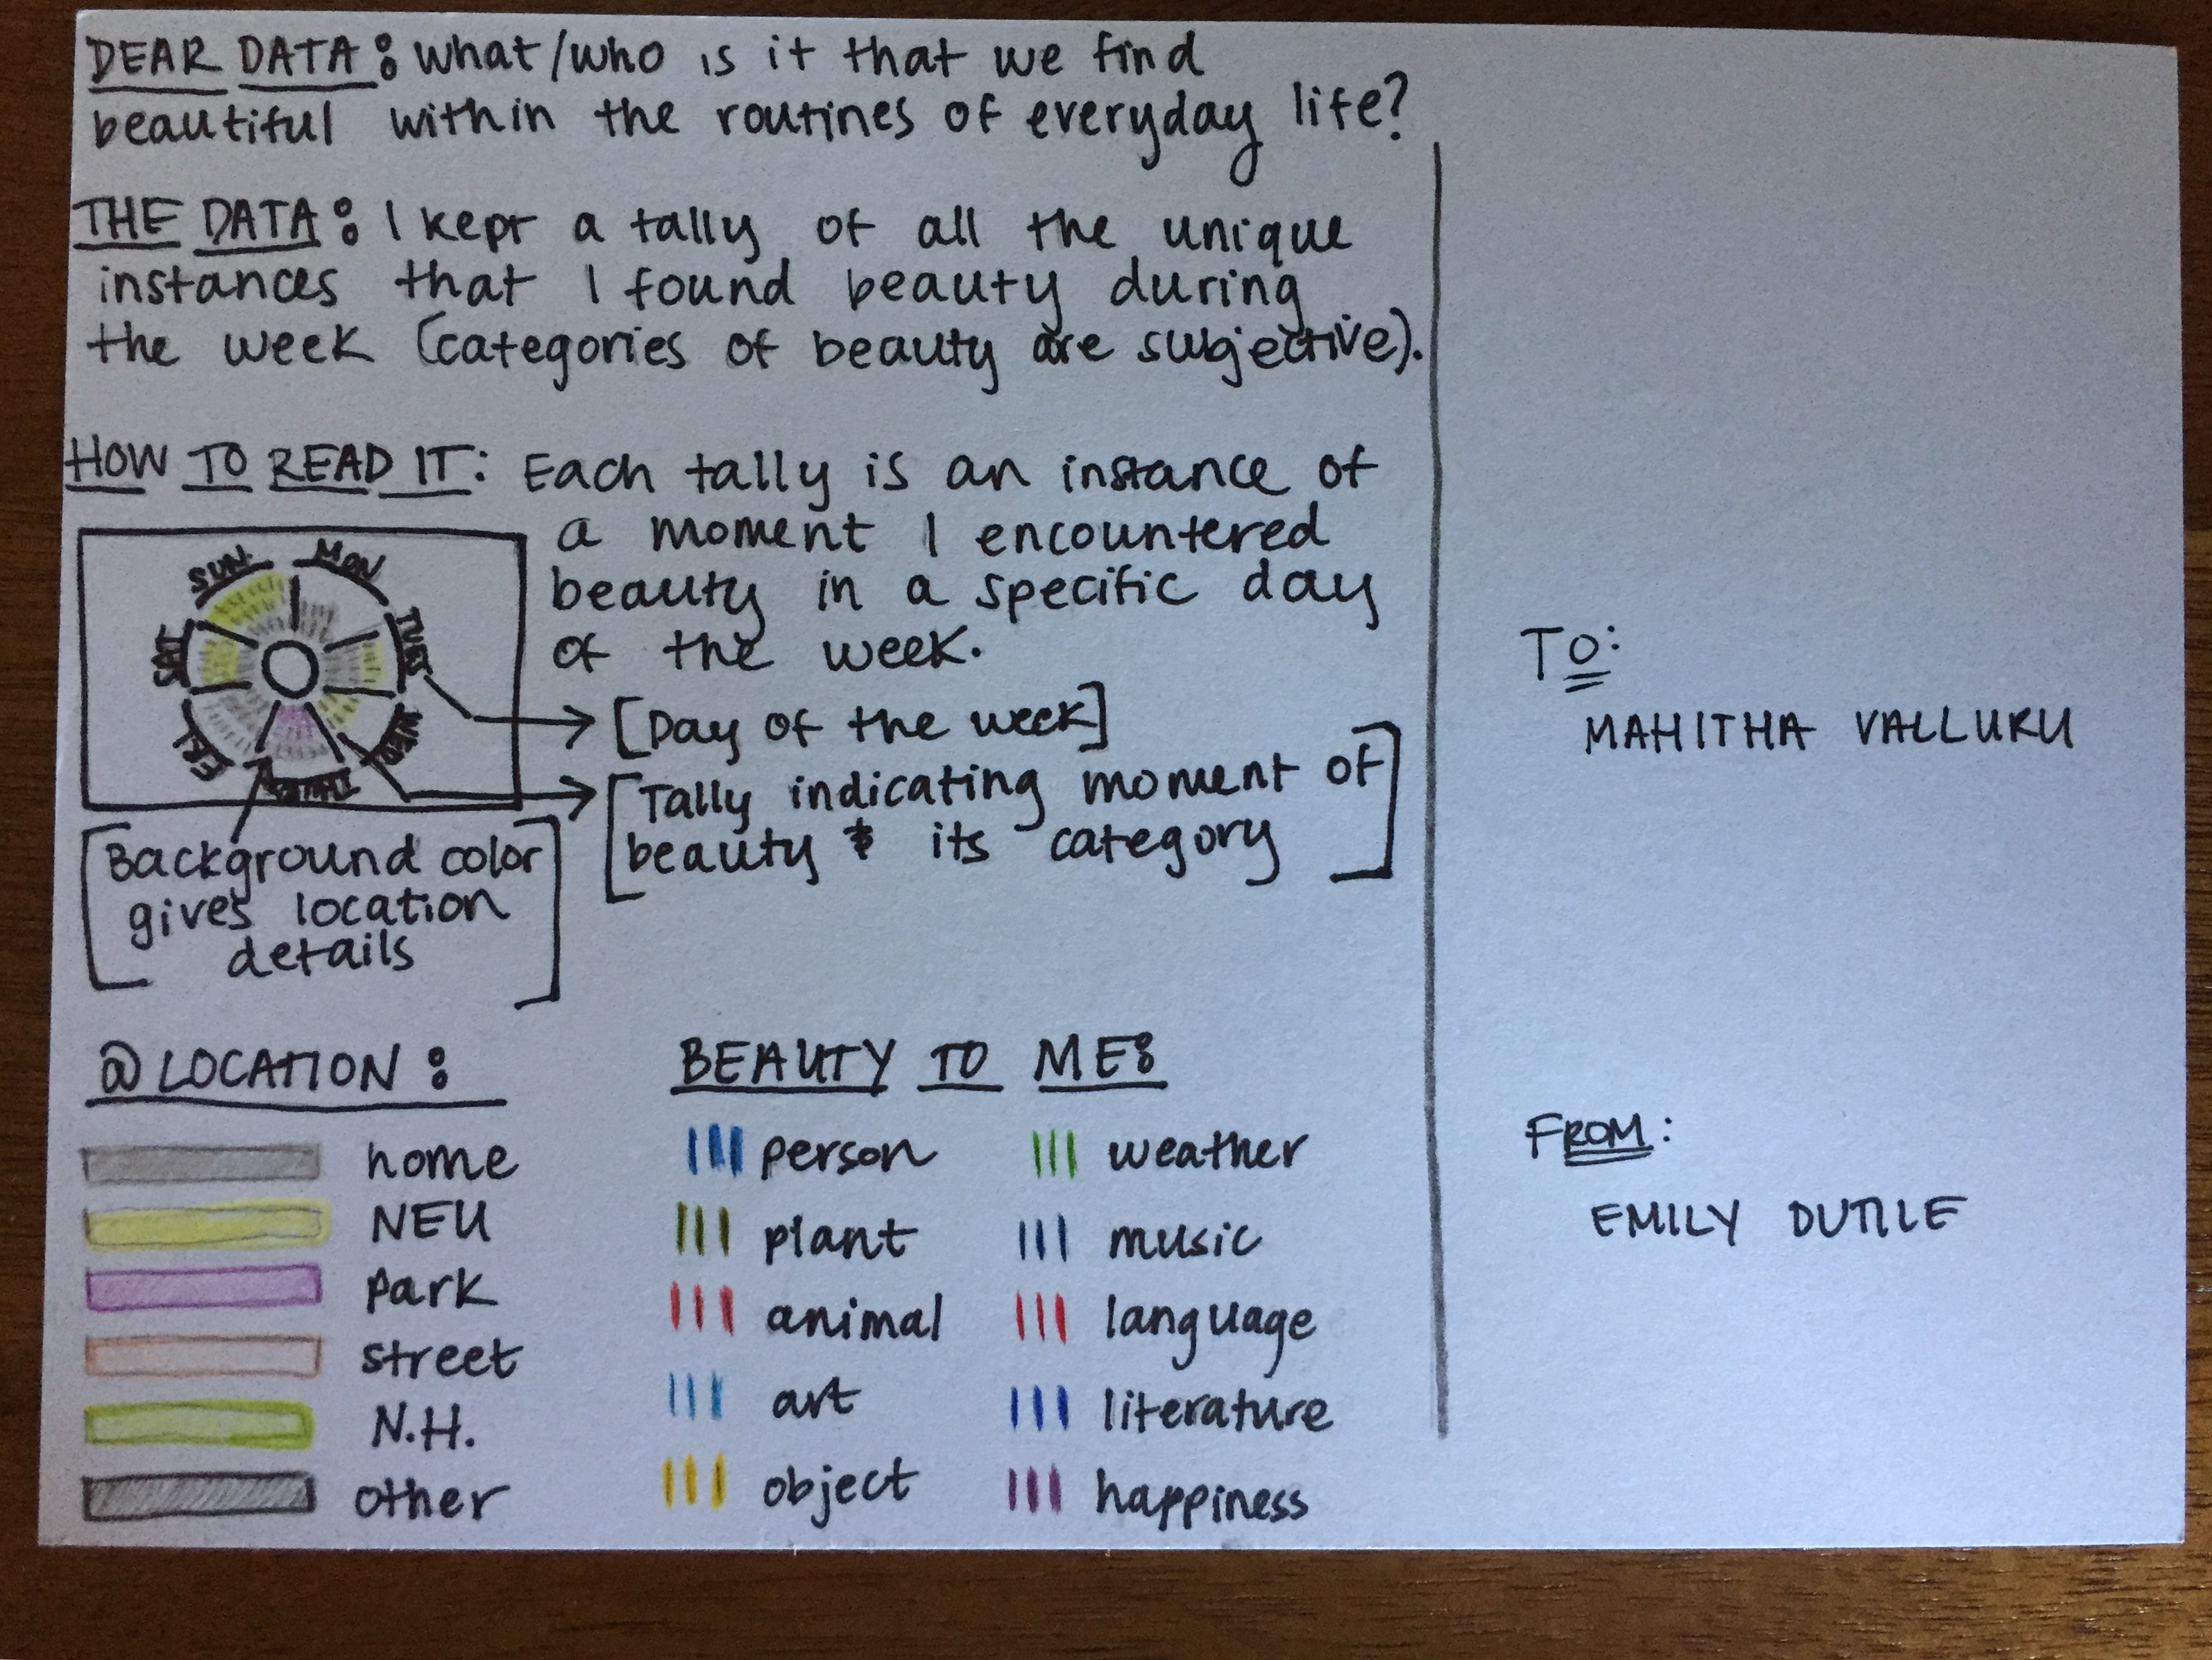
\includegraphics[width=0.4\linewidth]{myviz2}
}
\end{figure}

\subsection*{1.2 Pen Pal Visualization - Design “Critique”}

Mahitha Valluru visualized what/who she finds beautiful within the routines of everyday life by categorizing them by place, so she was either located in her apartment, on campus, or anywhere else in Boston. A lot of her observations took place in the apartment, however, she wished she noticed more while in the streets of Boston or near the Charles River.\\

Mahitha chose to use colors, shapes, and points for her marks and channels. I liked how she collected the data that she found to be beautiful that triggered one of her five senses, in order to make categorical data. It was a different and unique way of gathering data on "who/what is beautiful". Since she only used 3 colors to identify the 3 locations, it's easy to tell where she was when her observation of beauty occurred. I really like how she used distinct shapes to give insight into the specific observation, so the user has a better idea as to what Mahitha defines as beautiful. The definition of beautiful can be very subjective, so I really enjoyed this insight. I also thought the detail of the data was really nice, such as duration and reaction. I really liked the shapes of these two attributes. At a quick glance, I might have made the duration symbol between T and + and bit more distinct, but I think that's being overly picky. The shape of each data point was an interesting choice and I'd be curious to learn how it was chosen. I think I would have made the colors more contrasty/vibrant just to make them even more distinct, but for the sake of the assignment I know I was limited to my color choices as well. Overall I think it was a creative and effective visualization with the chosen color map.

\begin{figure}[h]
\centering
{
\includegraphics[page=2,width=0.4\linewidth]{penpal}
}
\end{figure}

\begin{figure}[h]
\centering
{
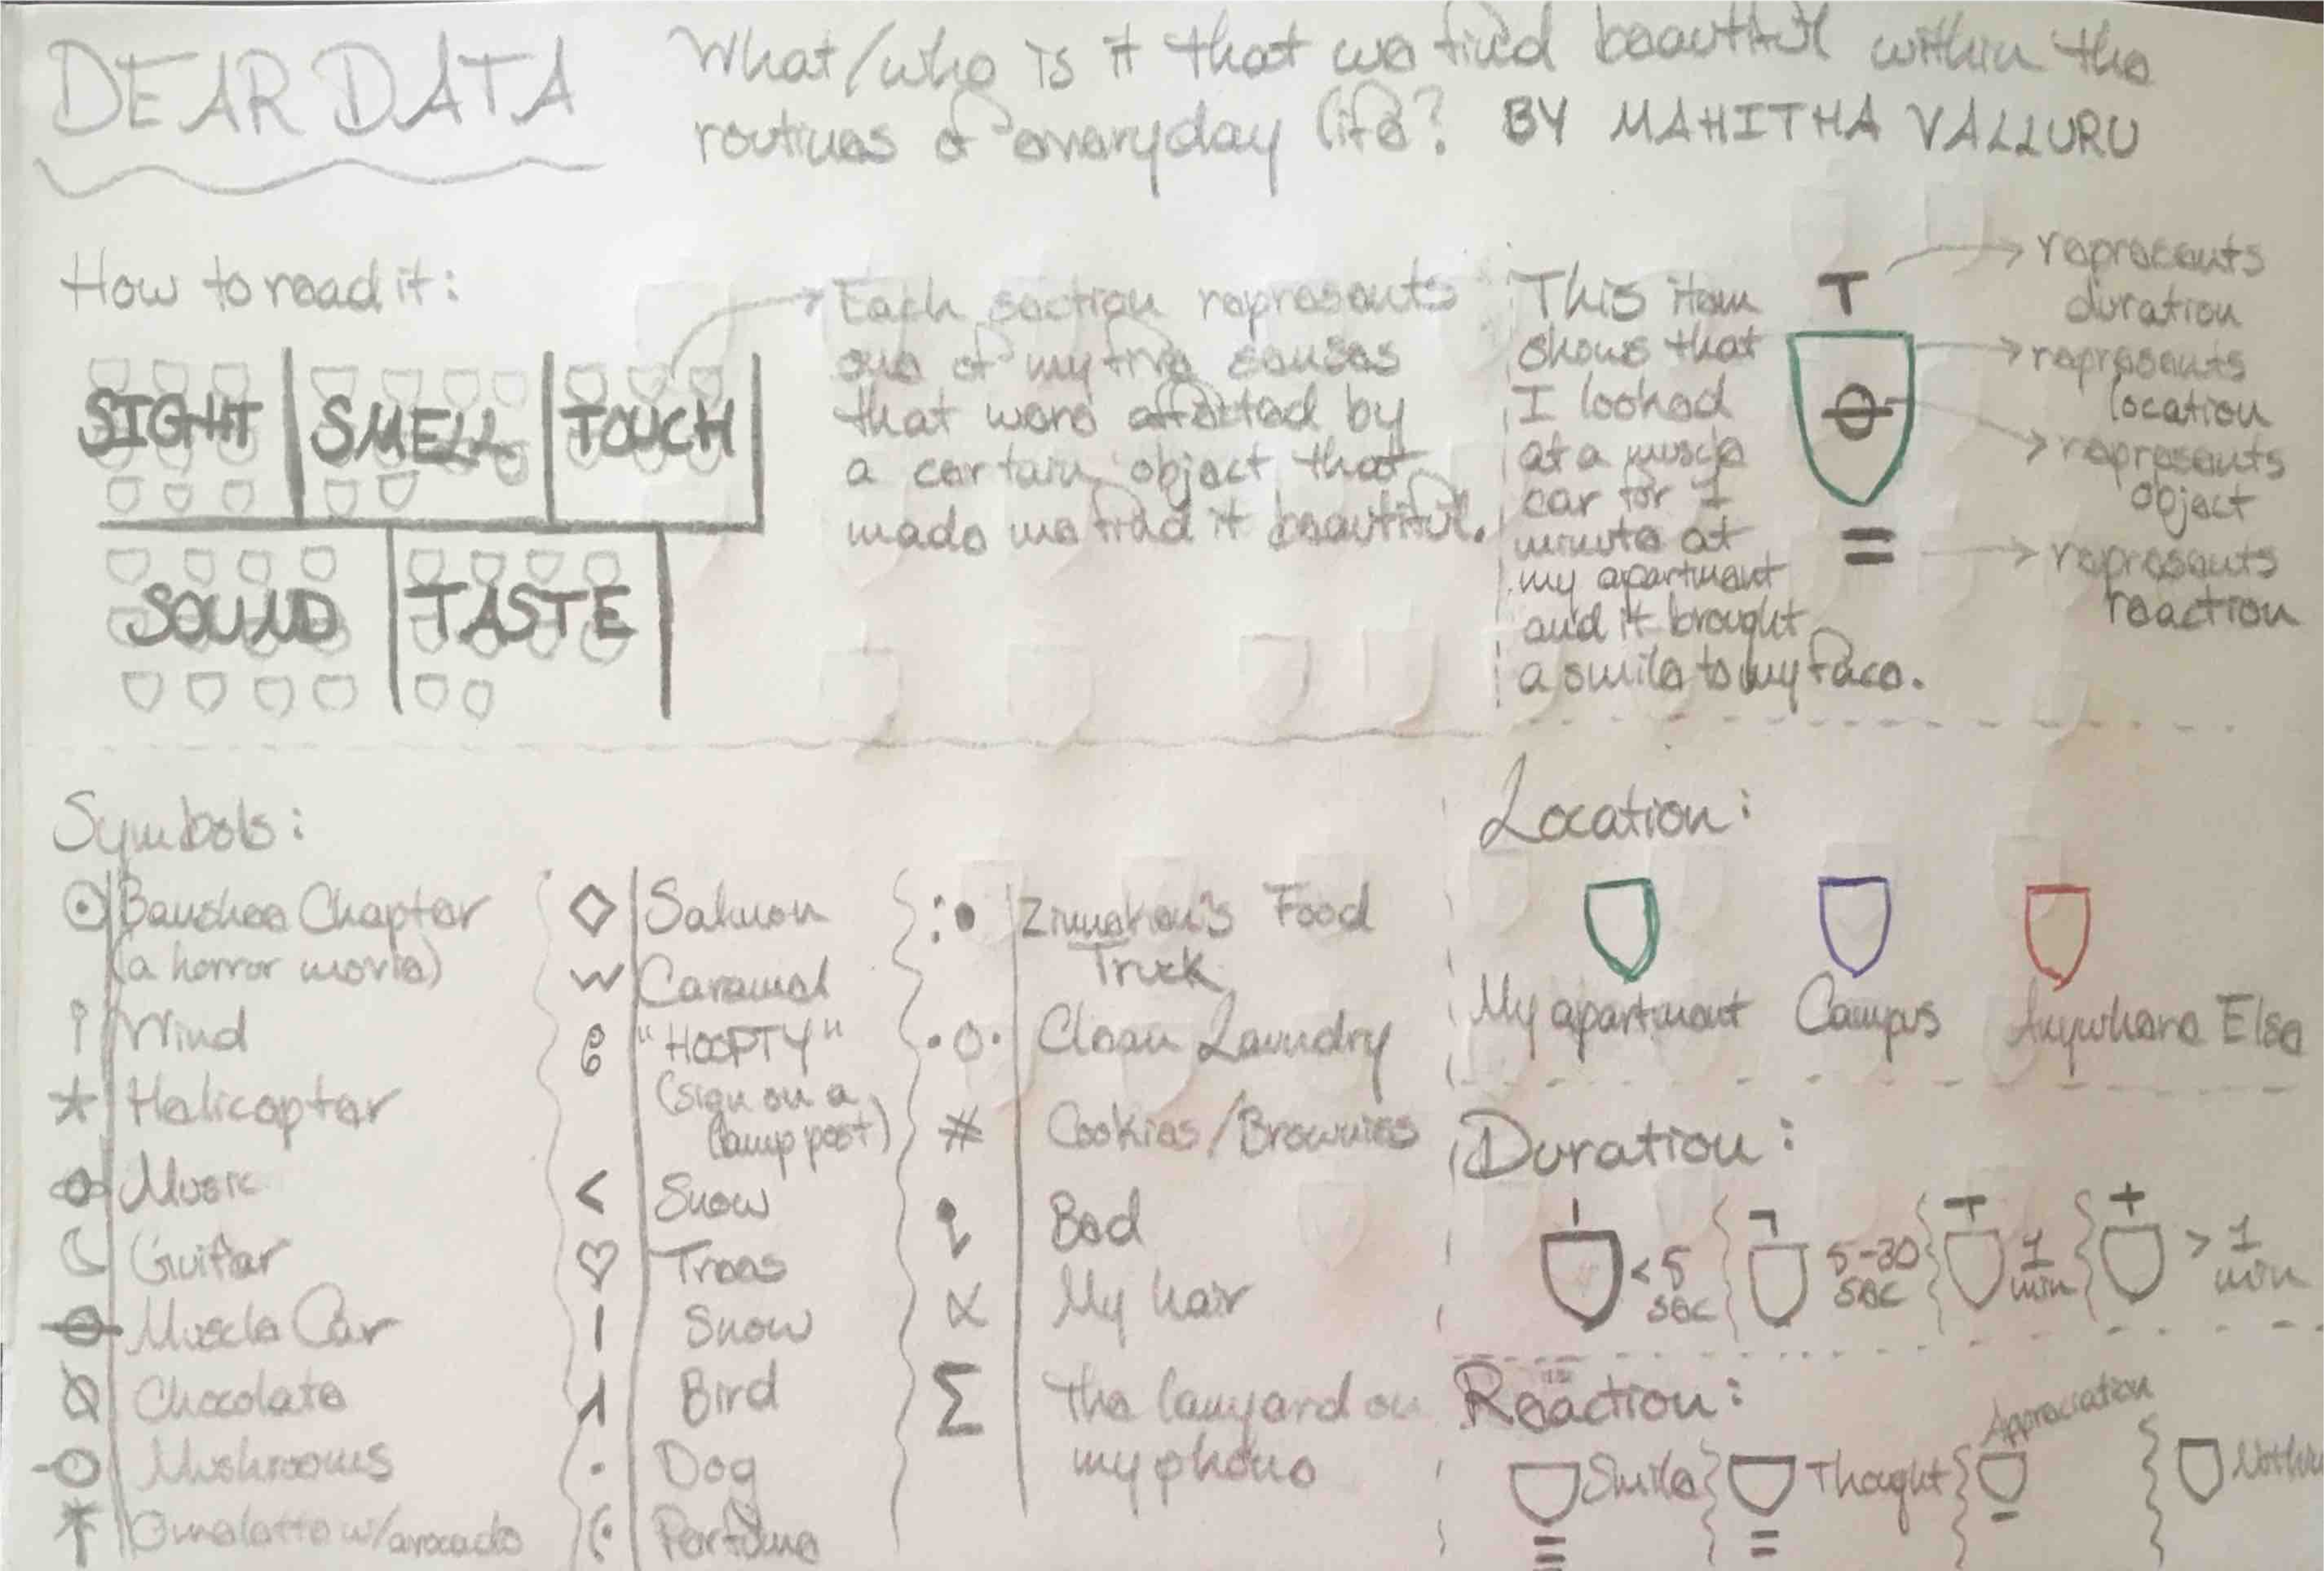
\includegraphics[page=1,width=0.4\linewidth]{penpal}
}
\end{figure}

\section*{2 Journal Paper Review – Color Theory Review}

\textbf{Did you learn anything reading this article new not discussed in class?  What concept you found most interesting in the article?}\\

I did learn a few new things that were not discussed in class. In general, I think we've hit the nail on the head with rainbow colormaps being bad. However, diving into the specifics of human perception and the unique examples was interesting. Having a really good understanding of our visual system as humans is extremely important when it comes to expressing our data appropriately in order to tell the accurate story. \\\\

\textbf{In a paragraph (few sentences): Pretend you are talking to a friend who is completely unfamiliar with data visualization and color theory.  Summarize the most important take-away messages from this article and in-class for practical advice on using and picking color for data visualizations and imaging.}\\

In summary, there are a few main points that should be taken away from the article. The authors go over a lot of things, but the main take away was the three perceptual dimensions – hue, saturation, and luminescence. The article presses the point that rainbow colormaps in general are usually (or almost always) bad, except for specific datasets. Second, for quantitative change, hue is not good to use either. Third, for low frequency change, saturation is usually good for this because humans perceive low frequency changes better in saturation variation. And finally, luminance is good for high frequency change because humans can perceive these changes better in this way. The first image presented really shows why we should greatly care about color as scientists because both images represent the same exact data and the only difference is in the color scale, but very different interpretations dependent on the colormap.

\section*{3 Boston Data Exploration}

Please see the iPython Notebook submitted in my NEU Google Drive (HW4-part3\_Dutile.ipynb).

\section*{4 D3 basics}

\subsection*{4.1 D3 a bar chart}

URL: https://jsfiddle.net/dutile/0a56q29g/2/ \\

In this visualization, I made a bar chart to count the number of homes by each ST name. Ideally, I would have liked to add in the names of the streets such as FENWAY on the x-axis, but I was running into issues with the sorting. The tooltip is not as "pretty" or ideal, seeing that it remains on the pages, but the value does update when the bar is hovered over for sake of requirements. \\\\

\subsection*{4.2 D3 scatter plot}

URL: https://jsfiddle.net/dutile/dgzfq1c9/6/ \\

The scatter plot shows the Boston neighborhoods by zip code on the x axis plotted with the number of properties in that zip code on the y axis (the count). Simple black and grey colors were used since there were only three categories (zipcodes) to keep it clean. On hover over, the selected bar turns grey and the count appears on demand.

\subsection*{4.3 D3 3/22 in class activity}

URL: https://jsfiddle.net/dutile/rbd58vkb/35/ \\

Scatter plot with tool tip




\end{document}
